% !TEX root= ../main.tex
\section{Results in Kernel Theory}
\label{sec:Results in Kernel Theory}
Ultimately, the end goal of Kernel Theory would be to have an easy way to answer the question "Does this digraph have a kernel?" no matter the graph, and no matter the answer.
We are not quite there, but a lot of work has been put into trying to identify special circumstances under which one is guaranteed to have (or guaranteed to not have) a kernel in the given graph.
One of the results is the Richardson's Theorem, worked out by Moses Richardson in 1953:\\

\begin{theorem}
  \cite{am-richardson} If D is a finitary\footnote{In a finitary graph, every vertex has a finite number of out-neighbors; the graph has finite branching.} digraph without odd cycles, then D has a kernel.
\end{theorem}
This theorem gives us the confirmation that whenever dealing with finitary dags, for instance, one can be certain that its corresponding theory is consistent.

Intuitively, one is tempted to believe that \textit{all} digraphs without odd cycles have kernels, but this is not the case.
Until now, our paradoxes have always been statements that -- directly or indirectly -- have been referring back to themselves (giving cycles in the graph) and thus causing a logical conflict, and it is hard to imagine any other way to construct paradoxical statements.
The following construction will however reveal our lack of imagination.

The \textbf{Yablo Graph} \cite{analysis-yablo} is an example of an acyclic graph with no kernel. It is constructed with an infinite set of vertices $\{ x_i | i \in \mathbb{N} \}$ and a set of edges $N$ such that $\langle x_i, x_j \rangle \in N$ iff $i < j$.
\[
  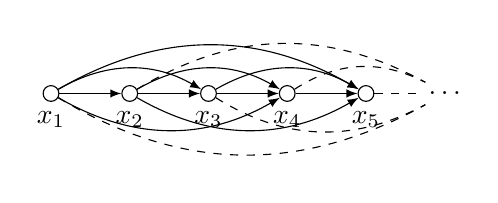
\begin{tikzpicture}
    [
    point/.style={circle,draw,inner sep=0pt,minimum size=2mm},
    collection/.style={thick,rectangle,draw,inner sep=0pt,minimum height=14mm, minimum width= 9mm}
    ]
    \node (1) at (0,1) [point,label=below:$x_1$] {};
    \node (2) at (1,1) [point,label=below:$x_2$] {};
    \node (3) at (2,1) [point,label=below:$x_3$] {};
    \node (4) at (3,1) [point,label=below:$x_4$] {};
    \node (5) at (4,1) [point,label=below:$x_5$] {};
    \node (6) at (5,1) [] {$\dots$};
    \draw [-latex] (1) to (2);
    \draw [-latex] (2) to (3);
    \draw [-latex] (3) to (4);
    \draw [-latex] (4) to (5);
    \draw [dashed] (5) to (6);
    \draw [-latex, bend left] (1) to (3);
    \draw [-latex, bend left] (2) to (4);
    \draw [-latex, bend left] (3) to (5);
    \draw [dashed, bend left] (4) to (6);
    \draw [-latex, bend right] (1) to (4);
    \draw [-latex, bend right] (2) to (5);
    \draw [dashed, bend right] (3) to (6);
    \draw [-latex, bend left] (1) to (5);
    \draw [dashed, bend left] (2) to (6);
    \draw [dashed, bend right] (1) to (6);
  \end{tikzpicture}
\]
Since there exist no two numbers $x,y \in \mathbb{N}$ such that $x < y$ and $y < x$, we get that the Yablo graph indeed is acyclic\todo{This is a bit over-simplified}.
Furthermore, since any natural number has infinitely many numbers strictly larger than it, we get that all the vertices are infinitely branching, making the Yablo graph infinitary (not finitary).

The corresponding discourse theory of the Yablo graph would -- informally -- be the situation with an infinite number of statements, all saying "Every statement after this statement is false".

We will later show that this graph is indeed without a kernel, but for now we will take Yablo's word \cite{analysis-yablo} for it.
